\documentclass[12pt,letterpaper]{article}

\usepackage[margin=0.75in,headheight=1.5em]{geometry}
\usepackage{graphicx}
\usepackage{tabu}
\usepackage{enumitem}
\usepackage[table]{xcolor}

\definecolor{thcolor}{RGB}{193,193,193}
\newcommand{\tableheader}{\rowfont\bf\rowcolor{thcolor!30}}

\begin{document}
    \begin{center}
        {\Large\bf Robot Evacuation} \\
        \vspace{0.25em}
        {\large COMP 4001}\\
        \vspace{0.25em}
        Juhandr\'{e} Knoetze - 100882772 \\
    \end{center}

    \section{Implementation}
    \subsection{Pygame}
        Pygame is a Python graphics library that provides a variety of objects for drawing and manipulating 2D objects. The two main objects utilized are the \texttt{Surface} and \texttt{Rect} objects. The \texttt{Surface} object is the object that gets drawn on. It holds the shapes and images that will be displayed to the screen. The \texttt{Rect} object is a the smallest (x, y) grid that represents a \texttt{Surface}. The \texttt{Rect} object of a \texttt{Surface} is the actual object that is manipulated and moved around the screen.
    
    \subsection{Classes}
        All the visual objects, such as \texttt{Ring} and \texttt{Robot} have \texttt{Surface} and \texttt{Rect} attributes. The \texttt{Rect} attributes are used to keeping track of the objects location as well as determining if there was a collision with another object or not.
    
    \subsubsection{Ring}
        The \texttt{Ring} object represents the ring the robots are trying to evacuate. A \texttt{Ring} has a \texttt{Surface} that has a circle drawn on to represent the perimeter of the ring. As well, it has a \texttt{Destination} object to represent the exit of the ring. 
        \newline
    
        \noindent Methods:
        \begin{itemize}
            \item \texttt{draw(surface)} \\
                \texttt{surface} is a Surface object. Draws the Ring on the given \texttt{surface}
            \item \texttt{pointOnRingAngle(angle)} \\
                \texttt{angle} is an angle in radians. It returns an (x,y) point on the perimeter of the Ring for the given \texttt{angle}
            \item \texttt{pointOnRing()} \\
                Returns a random point on the perimeter of the Ring
            \item \texttt{pointInRingAngle(angle)} \\
                \texttt{angle} is angle in radians. It returns an (x,y) point in the Ring that lies on the radius at the given \texttt{angle}
            \item \texttt{pointInRing()} \\
                Returns a random point inside the Ring
            \item \texttt{instersectionWithLine(line)} \\
                \texttt{line} is a Line object. Returns the points in which \texttt{line} intersects with the perimeter of the Ring
        \end{itemize}

    
%         \noindent
%         \begin{tabu} to \textwidth {>{\bf}l X}
%             \tableheader{}Method & Purpose \\
%             draw(surface) & \textit{surface} is a Surface object. Draws the Ring on the given \textit{surface} \\
%             pointOnRingAngle(angle) & \textit{angle} is an angle in radians. It returns an (x,y) point on the perimeter of the Ring for the given \textit{angle}\\
%             pointOnRing() & Returns a random point on the perimeter of the Ring \\
%             pointInRingAngle(angle) & \textit{angle} is angle in radians. It returns an (x,y) point in the Ring that lies on the radius at the given \textit{angle}. \\
%         \end{tabu}

    \subsubsection{Robot}
        The \texttt{Robot} class is used to represent the robots in the evacuation. In the \texttt{Robot} class, it has attributes to hold the visual representation of the \texttt{Robot}, as well as its coordinate location. There are also attributes to indicate if the robot has encounter the edge of the ring yet, or if it as evacuated. The \texttt{Robot} class also has a \texttt{Mask}. The \texttt{Mask} is a bit mask which is used for determining if a collision has a occurred with an object, such as a \texttt{Destination} object.
        
        \noindent Methods:
        \begin{itemize}
            \item \texttt{findPoint(pos, timeDelta)} \\
                \texttt{pos} is a an (x,y) coordinate and \texttt{timeDelta} is the change in time since the last frame in milliseconds. Moves the robot closer to the \texttt{pos} based on the \texttt{timeDelta} and returns whether it is on the \texttt{pos} or not.
            \item \texttt{collision(destination)} \\
                \texttt{destination} is an object that has a bitmask. It checks to see if the \texttt{destination} and robot have collided.
            \item \texttt{findExitOnRing(ring, timeDelta)} \\
                \texttt{ring} is the Ring object the robot is evacuating and \texttt{timeDelta} is the time since the last frame in milliseconds. It moves the robot around the \texttt{ring} until it finds the exit and returns whether it is on the exit or not.
            \item \texttt{drawRobot(surface)} \\
                \texttt{surface} is a Surface object. Draws the robot on the given \texttt{surface}
            \item \texttt{drawTravelled(surface)} \\
                \texttt{surface} is a Surface object. Draws a line representing the path the robot has traveled.
        \end{itemize}

    \subsubsection{Line}
        The \texttt{Line} class represents a line. It has a slope and a y-intercept. It does not have a visual component and is used solely for calculations involving lines.
    
        \noindent Methods:
        \begin{itemize}
            \item \texttt{fromPoints(point1, point2)} \\
                \texttt{point1} and \texttt{point2} are two (x,y) coordinates. It returns a new Line based on \texttt{point1} and \texttt{point2}
            \item \texttt{fromSlopeAndPoint(slope, point)} \\
                \texttt{slope} is the slope of a line and \texttt{point} is a point that is on that line. Returns a new Line based on the \texttt{slope} and \texttt{point}
            \item \texttt{findIntercept(point)} \\
                \texttt{point} is an (x,y) coordinate. It finds the y-intercept of the line using \texttt{point}
        \end{itemize}
        
    \subsection{Destination}
        The \texttt{Destination} class is a visual representation for a location on the grid.
                
        \noindent Methods:
        \begin{itemize}
            \item \texttt{draw(surface)} \\
                \texttt{surface} is a Surface object. Draws the Destination on the \texttt{surface}
        \end{itemize}

    \subsection{Button}
        The \texttt{Button} class is an object that uses an image to represent a button on the screen. \texttt{Button}s are triggered with the \texttt{MOUESUP} event.
        
        \noindent Methods:
        \begin{itemize}
            \item \texttt{eventHandler(event)} \\
                \texttt{event} is an Event object. Returns a function if the Button's event was triggered.
            \item \texttt{draw(surface)} \\
                \texttt{surface} is a Surface object. Draws the button on the \texttt{surface}
        \end{itemize}
        
    \subsection{REMain}
        The \texttt{REMain} class initializes the application. The initializes pygame to create the window of the application. As well, it holds the list of \texttt{Robot}s and the \texttt{Ring} that will be drawn on the screen. As well, it has a list of \texttt{Button}s for selecting the type of scenario to execute as well a list of \texttt{Button}s for running a given scenario once or fifty times.

        \noindent Methods:
        \begin{itemize}
            \item \texttt{setupCountButtons()} \\
                Initializes the list of \texttt{Buttons} for determining how many times to run a scenario.
            \item \texttt{setupScenarioButtons()} \\
                Initializes the lise of \texttt{Buttons} for handling what scenario to execute.
            \item \texttt{setupScenario1()} \\
                Initializes the start locations for the list of \texttt{Robot}s as well determines their destination to reach on the perimeter for the scenario where both robots start in the center. Returns the robots' first destination as an (x, y) coordinate.
            \item \texttt{setupScenario2()} \\
                Initializes the start locations for the list of \texttt{Robot}s as well determines their destination to reach on the perimeter for the  scenario only one robot starts in the center. Returns the robots' first destination as an (x, y) coordinate.
            \item \texttt{setupScenario3()} \\
                Initializes the start locations for the list of \texttt{Robot}s as well determines their destination to reach on the perimeter for the  scenario only one robot starts in the center. Returns the robots' first destination as an (x, y) coordinate.
            \item \texttt{setupRing()} \\
                Initializes the \texttt{Ring} that will be used for the robots to evacuate.
            \item \texttt{moveRobots(point, timeDelta)} \\
                \texttt{point} is an (x, y) coordinate and is the position on the perimeter the robots need to head for. \texttt{timeDelta} is the time since the last frame in milliseconds. Moves the \texttt{Robot}s in the \texttt{Ring} based on the \texttt{timeDelta}. Returns whether both \texttt{Robot}s have evacuated the \texttt{Ring} or not.
            \item \texttt{on\_init()} \\
                Initializes pygame and setups up the initial window \texttt{Surface} and gives it a background. It is the \texttt{Surface} that the \texttt{Robot}s and \texttt{Ring} will be positioned on.
            \item \texttt{main\_loop()} \\
                This is the main loop for the application.
        \end{itemize}

%         \noindent
%         \begin{tabu} to \textwidth {>{\bf}l X}
%             \tableheader{}Method & Purpose \\
%             findPoint(pos, timeDelta) & \textit{pos} is a an (x,y) coordinate and \textit{timeDelta} is the change in time since the last frame in milliseconds. Moves the robot closer to the \textit{pos} based on the \textit{timeDelta} and returns whether it is on the \textit{pos} or not \\
%             collision(destination) & \textit{destination} is an object that has a bitmask. It checks to see if the \textit{destination} and robot have collided \\
%             findExitOnRing(ring, timeDelta) & \textit{ring} is the Ring object the robot is evacuating and \textit{timeDelta} is the time since the last frame in milliseconds. It moves the robot around the \textit{ring} until it finds the exit and returns whether it is on the exit or not \\
%             checkDistance(point) & \textit{point} is an (x,y) coordinate. Returns the distance the center of the robot is from the \textit{point} \\
%             drawRobot(surface) & \textit{surface} is a Surface object. Draws the robot on the given \textit{surface} \\
%             drawTravelled(surface) & \textit{surface} is a Surface object. Draws a line of points the robot has travelled \\
%         \end{tabu}
        
    \section{Algorithms}
    \subsection{Scenario 1}
        In the first scenario, both robots start in the center of the ring. To start the search for the exit, both robots go in the same direction until the perimeter. Once at the perimeter, the robots will go around the perimeter in opposite directions. If either robot finds the exit, the other robot is notified and the first robot will stop moving. When a robot is notified that the other has found the exit, it cuts the chord. The notified robot will leave the perimeter and head in a straight line towards the first robot.
        
%         \begin{center}
%             \frame{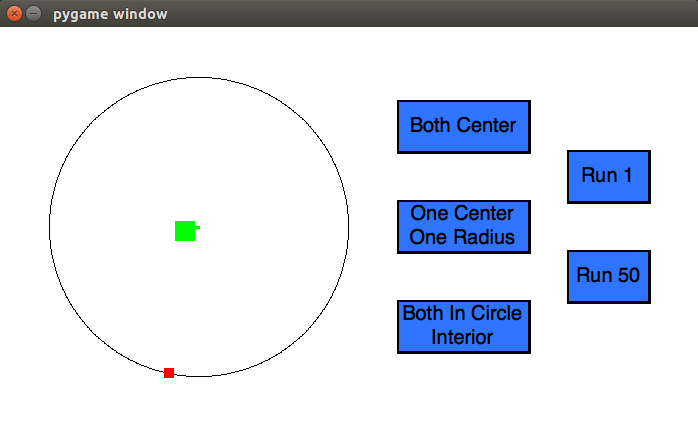
\includegraphics[scale=0.5]{images/scenario-1-1.png}}
%         \end{center}
%         
%         \begin{center}
%             \frame{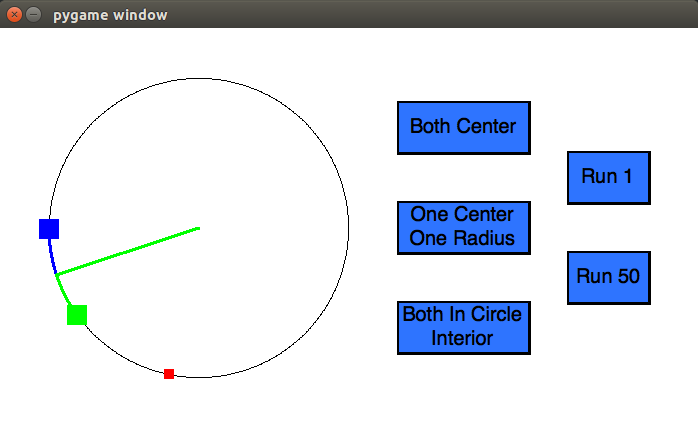
\includegraphics[scale=0.5]{images/scenario-1-2.png}}
%         \end{center}
%         
%         \begin{center}
%             \frame{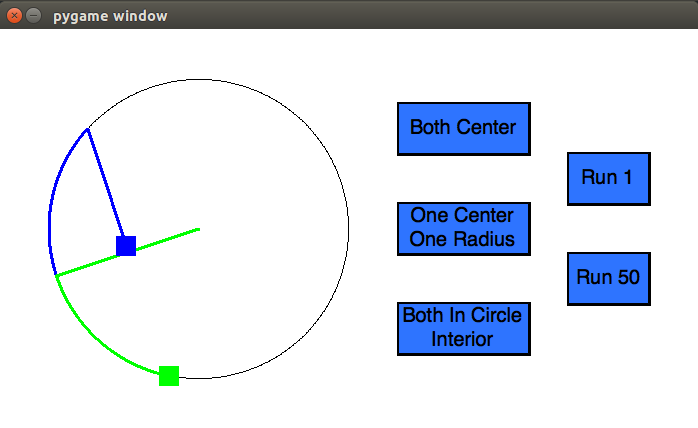
\includegraphics[scale=0.5]{images/scenario-1-3.png}}
%         \end{center}

        \begin{center}
            \frame{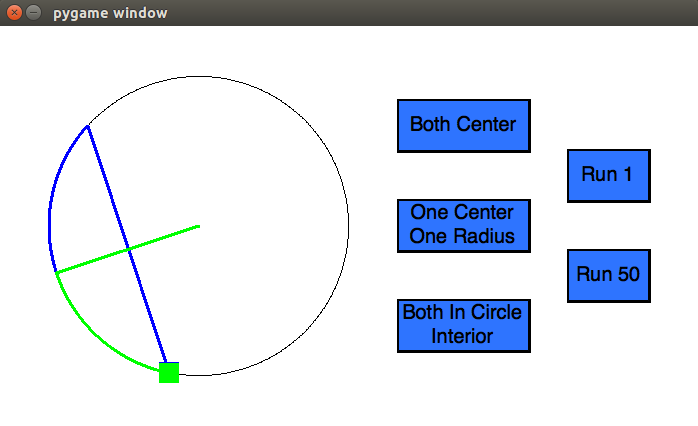
\includegraphics[scale=0.5]{images/scenario-1-4.png}}
        \end{center}

        \subsection{Scenario 2}
        In the second scenario, only one robot, robot $A$, will start in the center of the ring. The other, robot $B$, will be placed randomly in the ring. To evacuate the ring, both robots will go in the same direction towards the perimeter of the ring and start moving at the same time. The direction of travel will be such that robot $A$ is headed towards robot $B$. Since robot $A$ is in the center, it will always have to travel the radius of the ring regardless of where robot $B$ is placed. However, by traveling in that direction, robot $B$ will travel its shortest distance to the perimeter. Once the a robot reaches the perimeter, it will go in one direction and the other robot will always go in the opposite direction. This will ensure that the robots do not cover the same path along the radius, or else it would be equivalent to a single robot evacuation. Similarly to the first scenario, if a robot, say robot $A$, find the exit while searching the perimeter, it will stop moving and notify robot $B$. Robot $B$ will then cut the chord and head straight to the exit.
        
    
%         \begin{center}
%             \frame{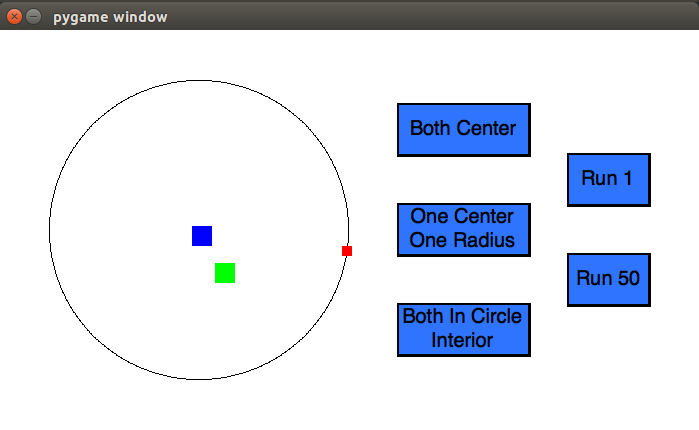
\includegraphics[scale=0.5]{images/scenario-2-1.png}}
%         \end{center}
%         
%         \begin{center}
%             \frame{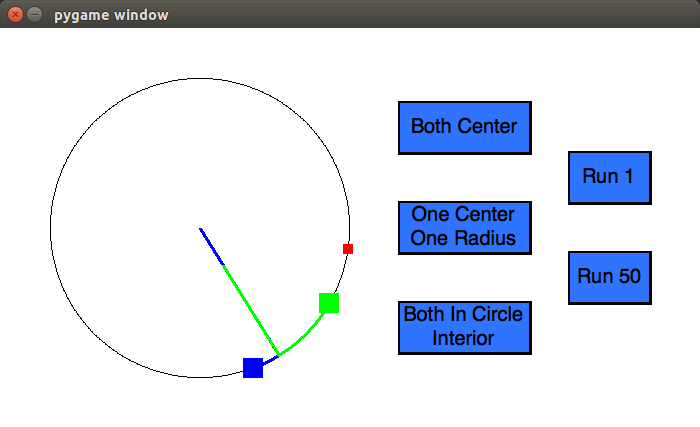
\includegraphics[scale=0.5]{images/scenario-2-2.png}}
%         \end{center}
%         
        \begin{center}
            \frame{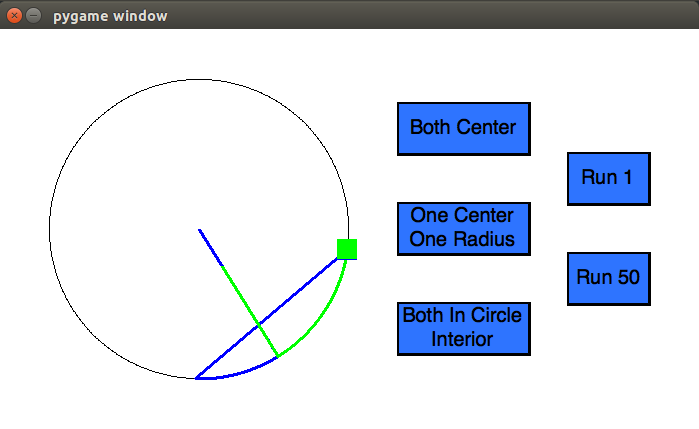
\includegraphics[scale=0.5]{images/scenario-2-3.png}}
        \end{center}
    
        The worst starting position for the robots would be if robot $B$ starts in the center with robot $A$. The farther robot $B$ starts away from the center, the less distance it has to travel to get to the exit. Therefore, starting at the center with robot $A$ would be worst case, which is just scenario 1.
        
    \subsection{Scenario 3}
        In the third scenario, both robots are placed randomly in the circle. To get to the perimeter, the robots head a to a point on the perimeter that is equidistant from both robots. To find this point, the line between the two robots is calculated as well as the midpoint of that line. With the midpoint and line, the line for the perpendicular bisector can be calculated. The perpendicular bisector will intersect the perimeter of the ring at either 1 or 2 points. If it is one point, the robots will head to that one point. If it is two points, the robots will head to the closet point. Once at the perimeter, the rest of the evacuation is identical to the other two scenarios. Both robots head in opposite directions and if one robot finds the exit, the other will cut across the circle to go to the exit.
        
%         \begin{center}
%             \frame{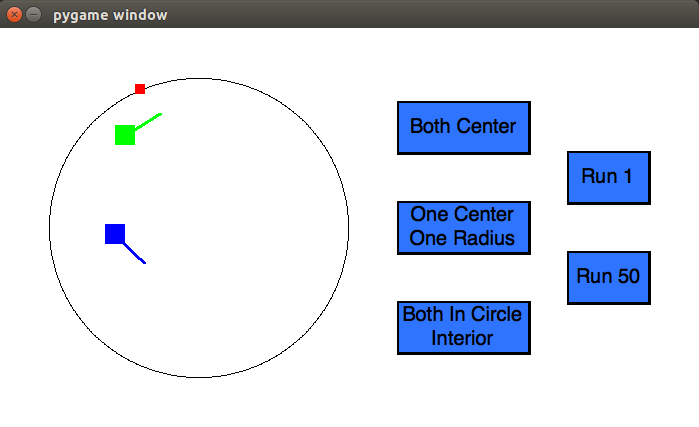
\includegraphics[scale=0.5]{images/scenario-3-1.png}}
%         \end{center}
%         
%         \begin{center}
%             \frame{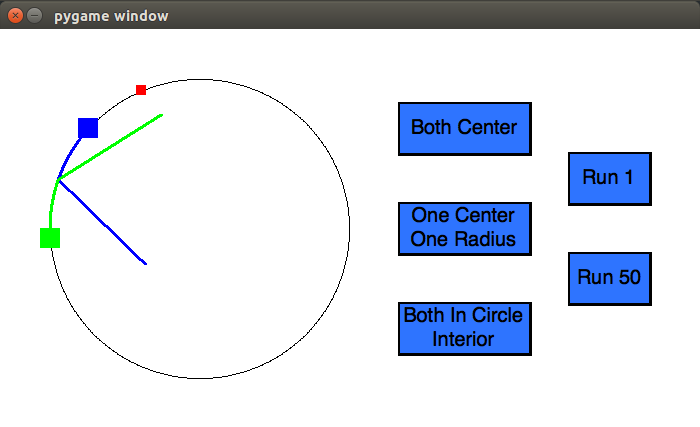
\includegraphics[scale=0.5]{images/scenario-3-2.png}}
%         \end{center}
%         
%         \begin{center}
%             \frame{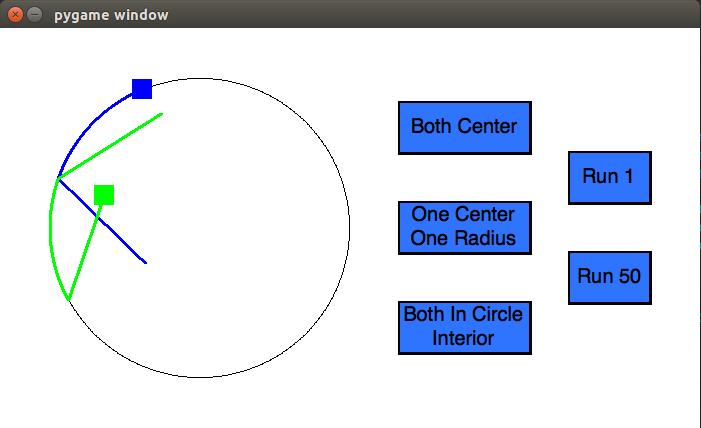
\includegraphics[scale=0.5]{images/scenario-3-3.png}}
%         \end{center}
%         
        \begin{center}
            \frame{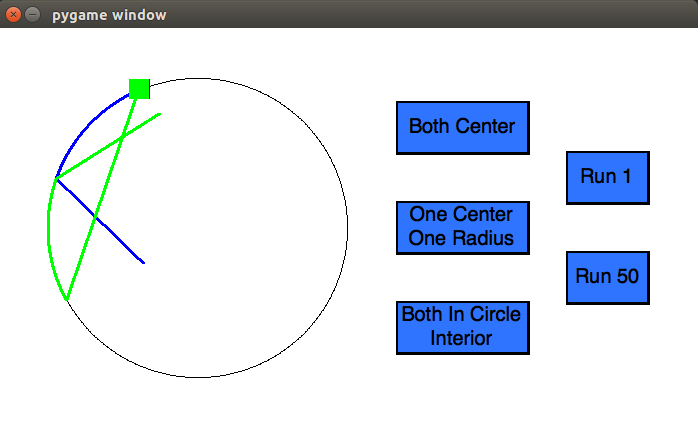
\includegraphics[scale=0.5]{images/scenario-3-4.png}}
        \end{center}
        
        The worst starting position for the two robots would be if they start a diameter apart on the perimeter. The point that is equidistant from both robots would then be $\sqrt{2}$.
        
        \begin{center}
            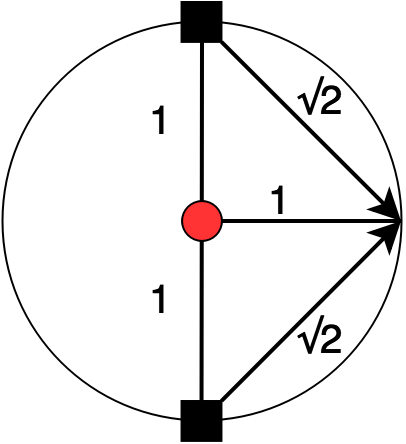
\includegraphics[scale=0.5]{images/scenario-3-worstcase.png}
        \end{center}
\end{document}